\section{Fourier Transform}

\subsection{Spectral Decomposition}

Fourier transforms constitute one of the most widely used tools for the analysis of turbulent flows and physical fields. The main idea consists in representing a signal as a superposition of sinusoidal modes associated with different spatial frequencies.

For a one- or two-dimensional scalar field $f(x,y)$, where $x$ and $y$ are the spatial coordinates, the Fourier transform is defined as


\begin{align}
    1D&: \hat{f}(k_x) = \int f(x) e^{-i k_x x} dx, \\
    2D&: \hat{f}(k_x,k_y) = \int\int f(x,y) e^{-i(k_x x + k_y y)} dx dy,  
\end{align}
where $(k_x,k_y)$ denote the spatial frequency components.

The Fourier transform can be interpreted as a projection of a signal onto a basis of globally supported sinusoidal functions. Therefore, the original field can be expressed as a linear combination of Fourier modes weighted by the corresponding spectral coefficients $\hat{f}(k_x,k_y)$. It is also possible to perform a non-linear reconstruction by retaining only the largest coefficients, as illustrated in Figure \ref{fig:fourier_decomposition}. The linear and non-linear reconstructions can be expressed as follows:

\begin{align}
    \text{Basis} &: F = \left\{ \phi_k \mid k\in\mathbb{Z},\ \phi_k(x) = e^{2\pi i k x} \right\}, \\
    \text{Linear} &: f_K(x)=\sum_{ |k| \le K }\langle f, \phi_k \rangle \phi_k(x), \\
    \text{Non-linear} &: f_H(x)=\sum_{ k \in \Lambda_H } \langle f,\phi_k \rangle \phi_k(x),
    \quad \Lambda_H=\left\{ k \mid |\langle f, \phi_k \rangle| \ge H \right\}.
\end{align}


\begin{figure}[ht]
    \centering

    \begin{minipage}{0.8\textwidth}
        \centering
        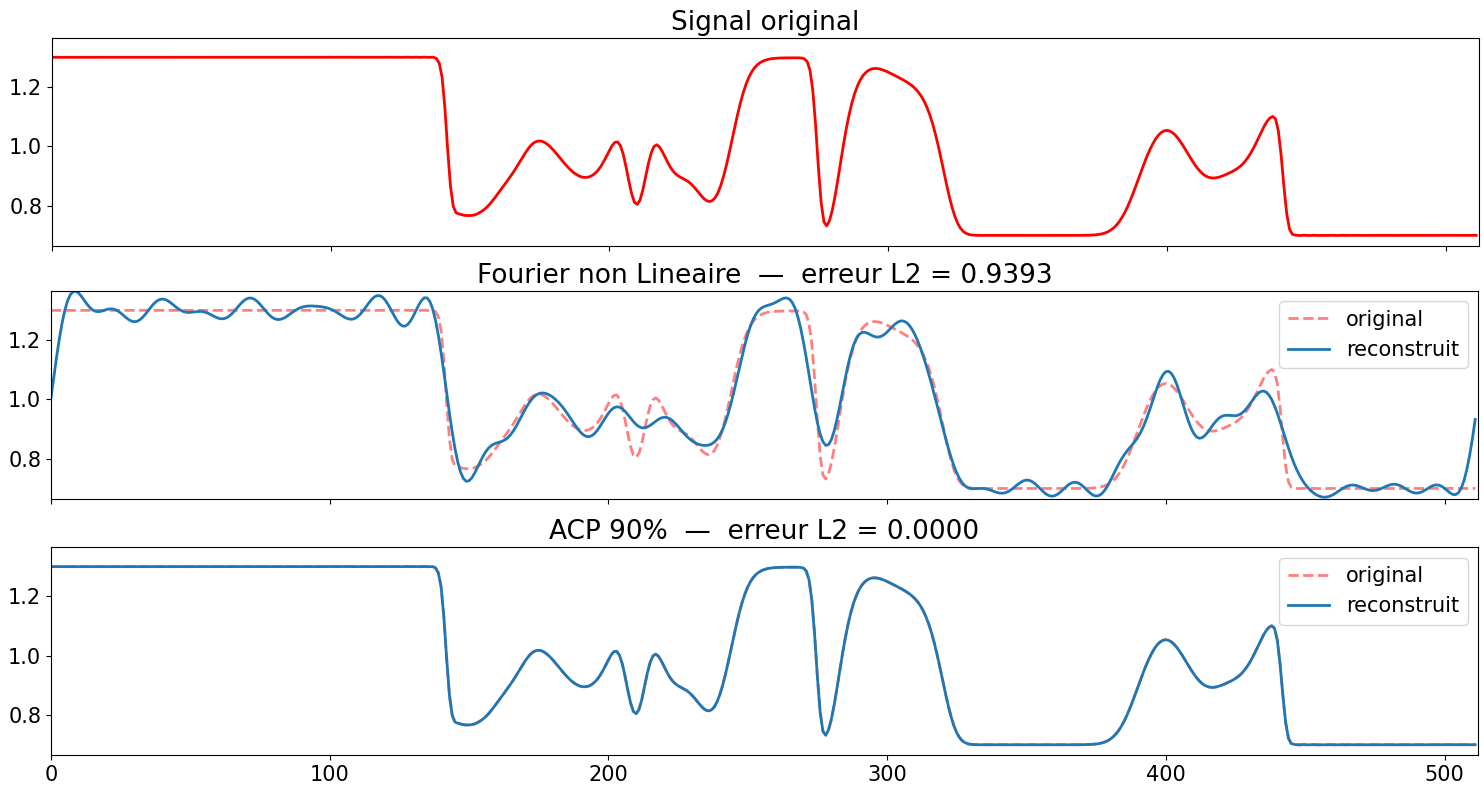
\includegraphics[width=\linewidth]{figures/ch2/sig.png}

        \vspace{0.3em}

        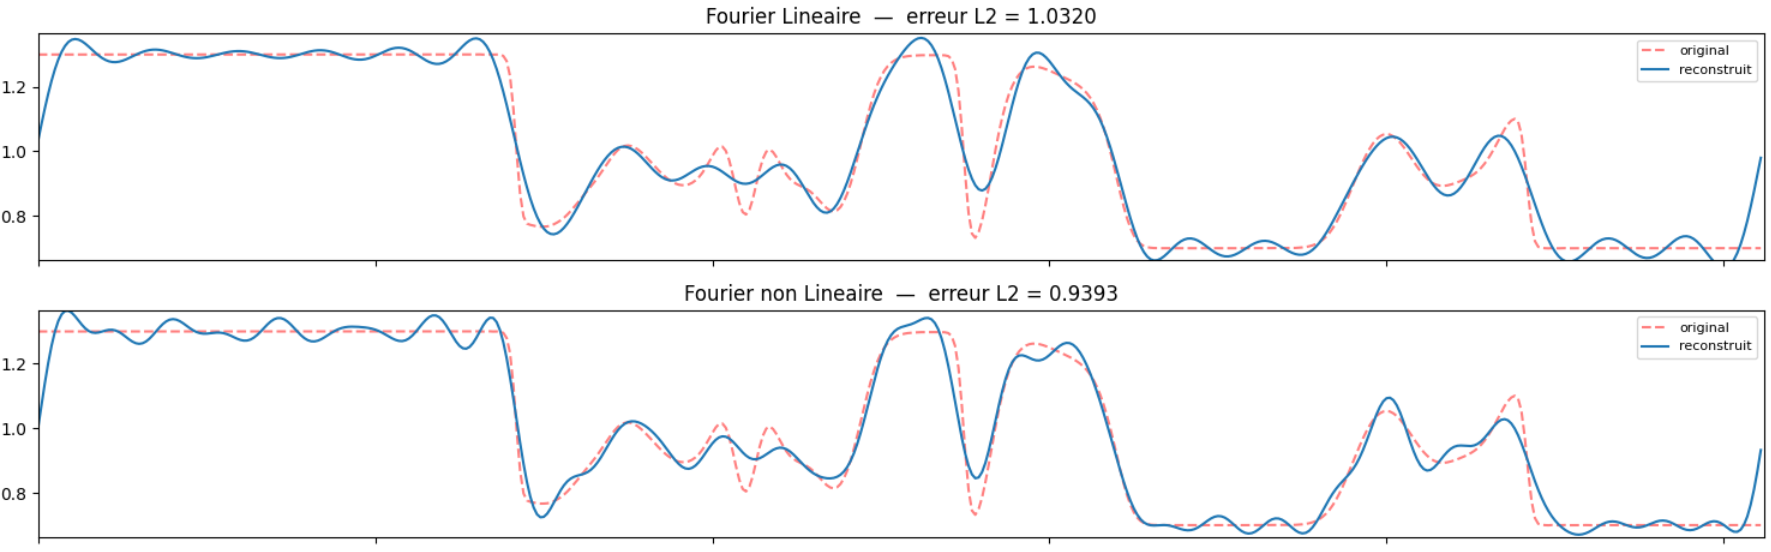
\includegraphics[width=\linewidth]{figures/ch2/fourier.png}
    \end{minipage}

    \caption{Illustration of a Fourier decomposition with 45 modes of a one-dimensional density field.}
    \label{fig:fourier_decomposition}
\end{figure}


In turbulence studies, Fourier analysis is particularly useful because it naturally describes the distribution of energy across spatial scales. Low-frequency modes correspond to large coherent structures, while high-frequency modes represent fine turbulent fluctuations.

\subsection{Advantages for Turbulence Analysis}

Spectral methods possess several important advantages for the analysis of fluid flows. First, Fourier transforms provide compact representations for smooth periodic signals. Second, many physical quantities of interest, such as energy spectra, can be directly expressed in spectral space.

In the context of DNS, pseudo-spectral solvers themselves are often formulated using Fourier representations because of their high numerical accuracy and low dissipation properties. Consequently, Fourier analysis naturally appears as a first candidate for dimensionality reduction and feature extraction.

Furthermore, spectral filtering techniques make it possible to separate structures according to their characteristic scales, which is particularly relevant for turbulent flows exhibiting cascade mechanisms.

\subsection{Limitations for Localized Structures}

Despite their numerous advantages, Fourier representations also exhibit important limitations when dealing with localized or non-smooth structures. Since Fourier basis functions extend over the entire spatial domain, local modifications of the signal affect all spectral coefficients simultaneously. As a consequence, sharp gradients and localized discontinuities generally require a large number of Fourier modes to be accurately reconstructed.

This limitation is closely related to the Gibbs phenomenon, which appears when truncated Fourier series are used to approximate signals containing discontinuities or strong localized variations. Near sharp interfaces, oscillatory artifacts emerge and persist even when increasing the number of retained modes, as shown in Figure~\ref{fig:gibbs}.

\begin{figure}[htbp]
\centering
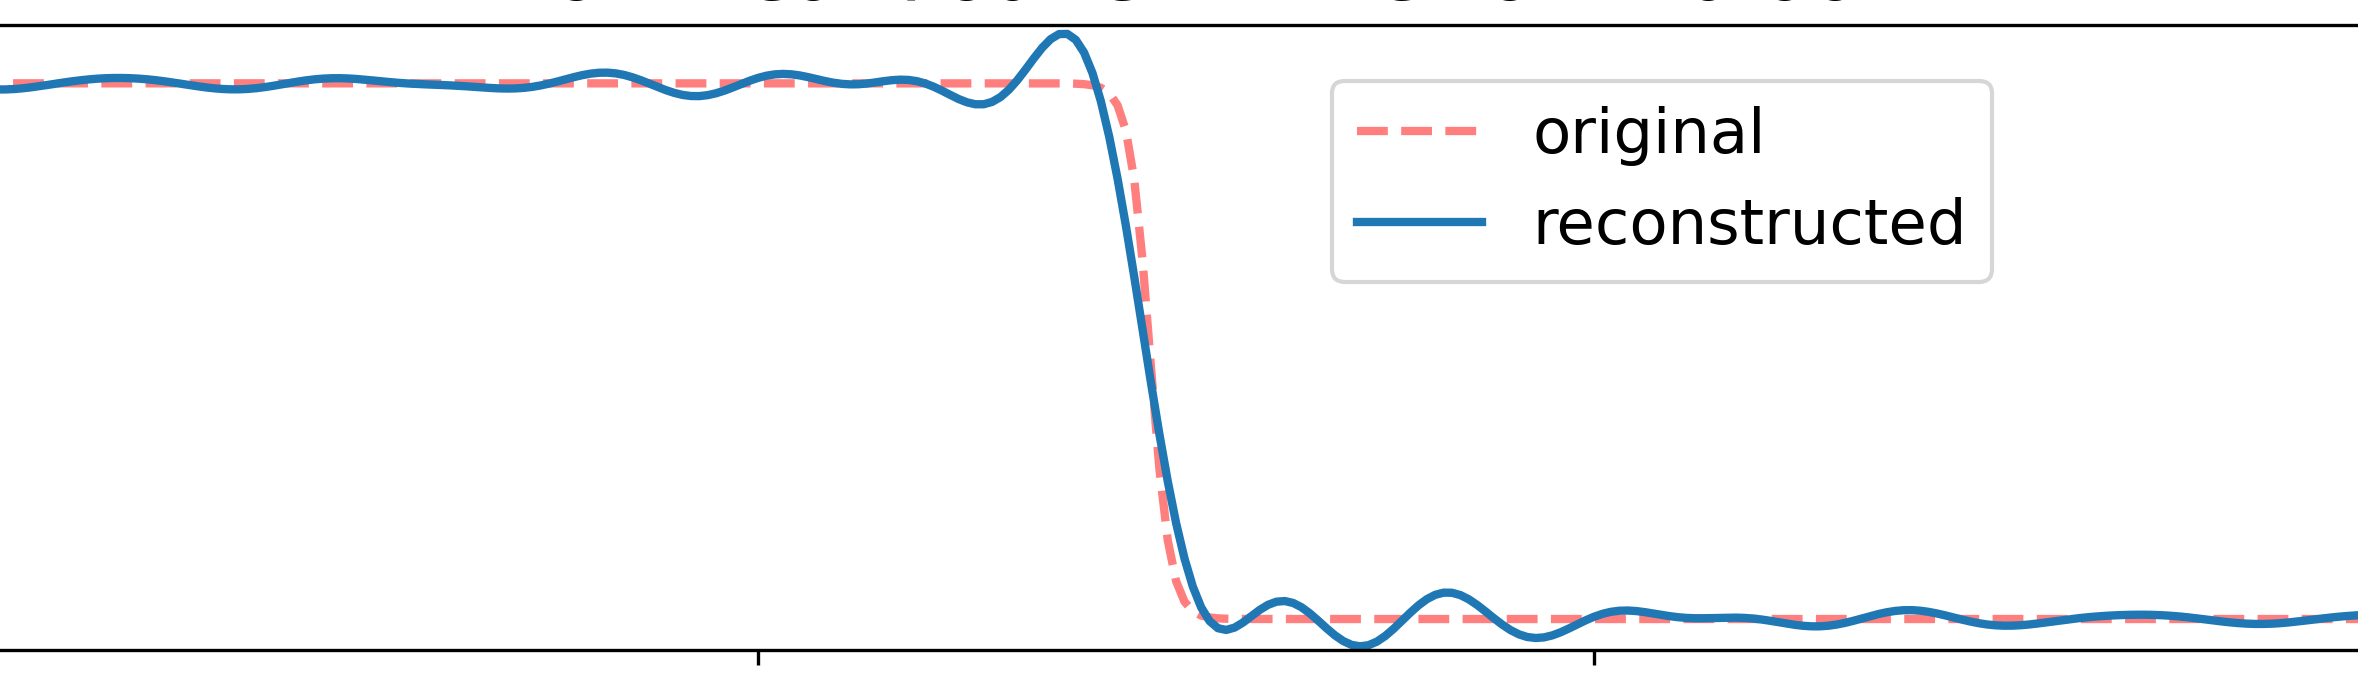
\includegraphics[width=0.65\textwidth]{figures/ch2/gibbs.png}
\caption{Illustration of the Gibbs phenomenon near a discontinuity reconstructed using a truncated Fourier representation.}
\label{fig:gibbs}
\end{figure}

Although RTI density fields are not strictly discontinuous, they contain steep density gradients, localized interface deformations, and intermittent turbulent structures that exhibit similar reconstruction difficulties. Capturing such localized features using Fourier modes may therefore require a large number of coefficients, reducing compression efficiency and increasing the complexity of the representation.

In addition, Fourier decompositions provide limited spatial localization information. While they accurately describe the global frequency content of the flow, they do not directly indicate where specific structures are located in physical space. This limitation becomes particularly important for turbulent RTI fields, where coherent structures and mixing regions evolve dynamically and remain strongly localized.

These observations motivate the investigation of multi-resolution approaches capable of simultaneously representing both scale-dependent information and spatial localization properties.

